\section{Bounds at any noise level, \texorpdfstring{$R_0$}{R0} in a random environment, and the lineage identity}\label{sec:bounds}

\paragraph{In brief.}
When host fluctuations have stable long-run statistics (conditions in Proposition~\ref{prop:bounds-any}), the linear rare-parasite ring gives an upper bound on threshold loss at every noise level. Environments independent in time cannot increase growth above the arithmetic-mean baseline. These results separate conclusions that hold for large fluctuations from those that require small noise.

Host fluctuations can be too large for second-order approximations. We therefore derive bounds at every noise amplitude and connect them to lineage sampling and the random-environment reproduction number $R_0^*$. Proofs are in Appendix~\ref{app:bounds}, with verification details in Online Resource~1.

\subsection{Bounds at any noise level, temporal independence, and the two means}\label{subsec:bounds-any}

The variational path principle \citep{dombry2011,kobayashi2017,sughiyama2019}, evaluated along two environment-independent Markov chains, bounds ring growth and threshold loss without small noise or geometric memory.

\begin{proposition}[All-noise ring bounds and equality cases]\label{prop:bounds-any}
Consider an $n$-stage ring with fixed staying contributions $0 \le s_k < 1$, baseline transfers $g_k > 0$, positive multipliers $h_k(t) > 0$ such that $(h_1(t), \dots, h_n(t))$ is jointly stationary and ergodic with $\E|\ln h_k(0)| < \infty$, and a positive initial amount in every stage ($x_k(0) > 0$). Set $\ell_k = -\E\ln h_k(0)$, $R_0 = \prod_{k=1}^n g_k/(1 - s_k)$, $\prod_{k=1}^n (\lambda - s_k) = \prod_{k=1}^n g_k$, $\mathcal{T} = \sum_{k=1}^n (1 - s_k/\lambda)^{-1}$, and $\mathcal{T}_0 = \sum_{k=1}^n (1 - s_k)^{-1}$.
\begin{enumerate}
\item[(a)] The long-run log growth rate $r = \lim_{t \to \infty} t^{-1}\ln X(t)$ exists almost surely, does not depend on the positive initial vector, and satisfies
\begin{equation}
r \ge \ln\lambda - \frac{1}{\mathcal{T}}\sum_{k=1}^n \ell_k, \qquad r \ge \frac{1}{\mathcal{T}_0}\left(\ln R_0 - \sum_{k=1}^n \ell_k\right).
\label{eq:bounds-growth}
\end{equation}
When $\E h_k(0) = 1$, $\ell_k \ge 0$ and $\mathbf{A}_0$ is the arithmetic-mean matrix; at any zero-growth divisor $R_0^*$ on $m$ counted birth transfers, $D = \ln R_0 - m\ln R_0^* \le \sum_{k=1}^n \ell_k$. For mean-one lognormal multipliers $h_k(t) = \exp(\sigma_k z_k(t) - \sigma_k^2/2)$ with unit-variance $z_k$, $\ell_k = \sigma_k^2/2$ for every autocorrelation, so $\mathcal{T}(\ln\lambda - r) \le \sum_{k=1}^n \sigma_k^2/2$, $D \le \sum_{k=1}^n \sigma_k^2/2$, and $\ln R_0 > \sum_{k=1}^n \sigma_k^2/2$ suffices for rare-parasite growth.
\item[(b)] For $n = 1$, $r = \E\ln(s_1 + g_1 h_1(0))$ exactly for any host memory, and $D$ solves $\E\ln[s_1 + (1 - s_1)\ee^D h_1(0)] = 0$. For any $n$ and any environment, $\liminf_{t \to \infty} t^{-1}\ln X(t) \ge \ln\max_k s_k$ whenever $\max_k s_k > 0$.
\item[(c)] Without staying ($s_k = 0$ for all $k$), both inequalities in Eq.~\eqref{eq:bounds-growth} and $D = \sum_{k=1}^n \ell_k$ hold with equality if the environment is ergodic under the $n$-step shift (mixing suffices), whereas one-step ergodicity alone does not suffice (for $n = 2$, $s_1 = s_2 = 0$, $g_1 = g_2 = 1$, and random-phase alternation between $(1.8, 0.2)$ and $(0.2, 1.8)$, $r = \ln 1.8$ exceeds the proposed equality value). Staying does not rule out equality across all stationary ergodic environments: in a two-stage ring with $s_1 \in [0, 1)$, $s_2 = 0$, independent standard Gaussians $Z_t$, $h_1(t) = \exp(\sigma Z_t - \sigma^2/2)$, and $h_2(t) = \exp(-\sigma Z_{t-1} - \sigma^2/2)$, $D = \sigma^2 = \ell_1 + \ell_2$ for every $s_1 \in [0, 1)$.
\end{enumerate}
\end{proposition}

\begin{figure}
\centering
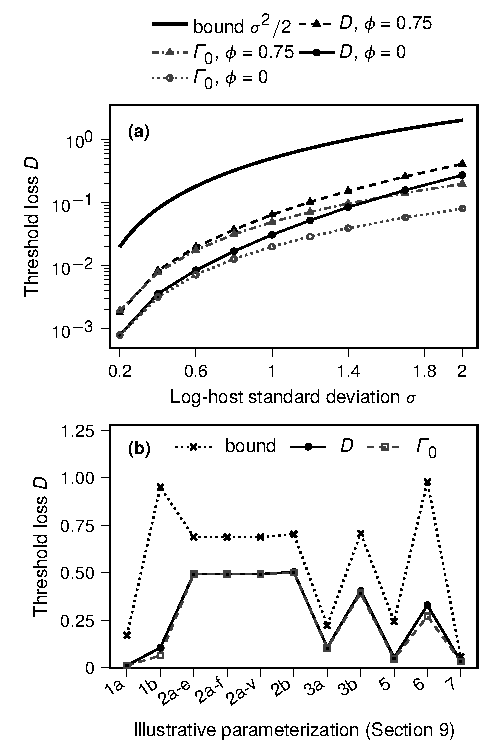
\includegraphics[width=84mm]{figures/bounds-1.pdf}
\caption{Simulated threshold loss $D$, second-order threshold approximation $\Gamma_0$, and all-noise upper bound $\sum_k \sigma_k^2/2$ in discrete-time lognormal $\mathrm{AR}(1)$ rings (simulation details in Online Resource~1). Panel~(a) shows stays $(1, 24)$ on a logarithmic vertical axis across $0.2 \le \sigma \le 2.0$ for $\phi = 0$ (simulated $D$, filled circles and solid line, and $\Gamma_0$, open circles and dotted line) and $\phi = 0.75$ (simulated $D$, filled triangles and dashed line, and $\Gamma_0$, open triangles and dash-dotted line), against the upper bound $\sigma^2/2$ (thick solid curve). Panel~(b) shows all 11 illustrative real-system parameterizations from Section~\ref{sec:num} in saved case order, comparing simulated $D$ (filled circles and solid line), second-order $\Gamma_0$ (open squares and dashed line), and the bound $\sum_k \sigma_k^2/2$ (crosses and dotted line), with connecting lines guiding the eye across categorical cases and simulation standard errors ($\le 0.0007$) smaller than the symbols}
\label{fig:bounds-1}
\end{figure}

Stage durations do not enter the worst-case bound, which cannot be sharpened over all stationary ergodic environments. Simulated cycles with a long steady stage remained below it at large noise, while exceeding $\Gamma_0$ (Fig.~\ref{fig:bounds-1}). This comparison does not prove $\Gamma_0 \le D$ at every noise level. The 161-case campaign and worked values are in Online Resource~1.

Temporal independence of the whole projection matrix rules out growth above the arithmetic-mean matrix baseline \citep{cohen1979b,tuljapurkar1990}.

\begin{proposition}[Environments independent in time give nonnegative loss]\label{prop:bounds-iid}
Let $\mathbf{x}(0)$ be an almost surely nonzero nonnegative vector with finite expectation, and let $(\mathcal{F}_t)_{t\geq0}$ be a filtration such that $\mathbf{x}(0)$ is $\mathcal{F}_0$-measurable, $\mathbf{A}(t)$ is $\mathcal{F}_{t+1}$-measurable, and $\E[\mathbf{A}(t)\mid\mathcal{F}_t]=\mathbf{A}_0$ for all $t\geq0$ with finite nonnegative $\mathbf{A}_0$ (in particular, when $\mathbf{x}(0)$ and $\mathbf{A}(0),\mathbf{A}(1),\dots$ are mutually independent with mean $\mathbf{A}_0$). Then $\E\mathbf{x}(t)=\mathbf{A}_0^t\E\mathbf{x}(0)$ and $\limsup_{t\to\infty}t^{-1}\ln\|\mathbf{x}(t)\|_1\leq\ln\spr(\mathbf{A}_0)$ almost surely, with $\ln0=-\infty$. For a restoring birth multiplier $\ee^y$ relative to a mean threshold, assume additionally that for every $y<0$ the tilted matrices $\mathbf{A}_y(t)$ are $\mathcal{F}_{t+1}$-measurable with $\E[\mathbf{A}_y(t)\mid\mathcal{F}_t]=\mathbf{A}_0(y)$ and $\spr(\mathbf{A}_0(y))<1$. Every finite zero-growth root then has $\Delta\geq0$. In particular, $D\geq0$ in the fixed-staying ring at every existing root $R_0^*$.
\end{proposition}

\begin{remark}\label{rem:bounds-pairwise}
Proposition~\ref{prop:bounds-iid} allows arbitrary same-step dependence among entries of $\mathbf{A}(t)$ and does not assert strict positivity $D > 0$. However, zero autocorrelation of each host at nonzero lags does not replace independence of the whole matrix from its past. In Appendix~\ref{app:bounds} we record a strictly positive two-stage matrix family driven by fair signs that are pairwise independent across all distinct times yet dependent in triples, for which $r = \sigma^3/3 + O(\sigma^4) > 0 = \ln\lambda(\mathbf{A}_0)$ for small $\sigma > 0$ (derived once in referee checks).
\end{remark}

Together, Propositions~\ref{prop:bounds-any} and~\ref{prop:bounds-iid} show why comparisons depend on which mean host abundance is held fixed.

Effective circuit reproduction is bounded below by its geometric-mean-host value and, under temporal independence, above by its arithmetic-mean-host value (Corollary~\ref{cor:bounds-means}, Appendix~\ref{app:bounds}).

Without staying in a mixing environment, effective circuit reproduction equals the geometric-mean-host value. With staying and temporally independent matrices, it lies between the geometric- and arithmetic-mean-host values. These bounds do not imply monotonicity as a stay changes. Field comparisons therefore require a specified common mean (numerical examples in Online Resource~1).

\subsection{The reproduction number in a random environment}\label{subsec:bounds-r0star}

\citet{bacaer2013} characterize reproduction in a finite-state Markov environment by the common birth divisor that reduces long-run growth to zero. We use this characterization to define $R_0^*$ in the Gaussian ring.

\begin{proposition}[Existence, invariance, and threshold expansion of $R_0^*$]\label{prop:bounds-r0star}
Fix staying contributions $0 \le s_k < 1$ ($n = 1$, or $n \ge 2$ with at least one $s_k > 0$), mean transfers $g_k > 0$, mean-one lognormal multipliers from stationary Gaussian $\mathrm{AR}(1)$ drivers ($|\phi_k| < 1$), and $1 \le m \le n$ transfers counted as births.
\begin{enumerate}
\item[(a)] Without noise, the next-generation reproduction number $\spr(\mathbf{F}(\mathbf{I} - \mathbf{V})^{-1})$ is $R_0^{1/m}$, with threshold $R_0 = 1$ for every $m$, and $\ln\lambda = \ln R_0 / \mathcal{T}_0 + O((\ln R_0)^2)$ as $\ln R_0 \to 0$ at fixed stays (exact at every $R_0$ when $n = 1, s_1 = 0$).
\item[(b)] There exists a unique divisor $R_0^* > 0$ on the $m$ birth transfers at which $r = 0$, the population grows when rare ($r > 0$) if and only if $R_0^* > 1$, and
\begin{equation}
m\ln R_0^* = \ln R_0 - D,
\label{eq:bounds-r0star}
\end{equation}
where $D$ depends only on the stays $s_k$ and the joint driver law, and depends neither on the mean transfers $g_k$ nor on $m$.
\item[(c)] Scaling noise along a fixed direction $\sigma_k = \sigma\eta_k$ (with $s_k$, $\eta_k$, driver assignments, and $\phi_k$ fixed), put $\tau_{k,0} = 1/(1 - s_k)$ and $\mathcal{T}_0 = \sum_{k=1}^n \tau_{k,0}$, and let $\Gamma_0 = \mathcal{T}_0 C_0 \sigma^2$ be the second-order per-generation loss evaluated at $\lambda = 1$. Then $D = \Gamma_0 + o(\sigma^2)$ by convexity alone, and $|D - \Gamma_0| \le K'\sigma^4$ for $|\sigma| \le \sigma_0$ by Lemma~\ref{lem:ring-rem-uniform}. For independent hosts with $0 \le \phi_k < 1$,
\begin{equation}
\Gamma_0 = \sum_{k=1}^n \sigma_k^2 \left[ \frac{1 + 2\theta_k}{2\mathcal{T}_0} - \frac{R_{k,0}}{1 - R_{k,0}} \right], \qquad R_{k,0} = \prod_{j=1}^n \frac{1}{1 + \tau_{j,0}/\theta_k} \quad (R_{k,0} = 0 \text{ at } \phi_k = 0).
\label{eq:bounds-gamma0}
\end{equation}
\end{enumerate}
\end{proposition}

Counting all transfers as births divides $\ln R_0$ and $D$ equally, leaving the invasion threshold unchanged. Away from $R_0 = 1$, $\Gamma_0$ uses threshold stays $\tau_{k,0} = (1 - s_k)^{-1}$, not lineage stays $\tau_k = (1 - s_k/\lambda)^{-1}$. Transfer invariance of $D$ does not extend to growth variance $V$. A numerical check is in Online Resource~1. In continuous time, this formal normalization matches \citet{bacaer2007} at a single frequency, without a proved remainder.

\subsection{Lineage representation, the variance identity, and its literature status}\label{subsec:bounds-lineage}

Weighting each transition's expected logarithmic penalty $\ell_e = -\E\ln h_e(0)$ by how often a reference lineage uses it gives an upper bound on growth loss for general life cycles (Proposition~\ref{prop:bounds-path}, Appendix~\ref{app:bounds}). The gap $\ell_e$ equals $\sigma_e^2/2$ (transition log standard deviation $\sigma_e$) unconditionally only for mean-one lognormal multipliers (counterexample in Online Resource~1).

To second order, growth loss equals this visit-weighted bound minus half the within-environment variance rate among coexisting lines of descent, so differing lineage histories reduce the penalty (Theorem~\ref{thm:bounds-lineage}, Appendix~\ref{app:bounds}).

The lineage variance in Theorem~\ref{thm:bounds-lineage} is the within-environment variance among reference lineages, averaged over environments and expressed as a long-run rate. It differs from population growth-rate variance and requires primitivity. Simulations agreed within sampling error across eight primitive models (details in Online Resource~1). Comparing life cycles requires a common unit for loss, because the mean penalty, generation time, and mean matrix can all change.

\paragraph{Literature status.}
We claim no priority or new mathematics for Proposition~\ref{prop:bounds-path} or Theorem~\ref{thm:bounds-lineage}. The former is a direct corollary of published results, and the latter rewrites a published perturbation coefficient. The reference chain and edge elasticities appear in \citet{bienvenu2017}, path representations and Jensen bounds in \citet{dombry2011,kobayashi2015,kobayashi2017}, and lineage cumulant expansions in \citet{nozoe2017,levien2020a,genthon2021,yamauchi2022}. The random-environment coefficient is due to \citet{tuljapurkar1982a,tuljapurkar1990,tuljapurkar2006}. Our 28-work review did not find Eq.~\eqref{eq:bounds-lineage} in this variance form with its total-variance equivalence to $C''$. Three supplements and four full texts remained unavailable. The reading record and related literature are in Online Resource~1.

For a parasite in the fixed-staying ring, the aggregate threshold loss satisfies $D\leq\sum_k\ell_k$ at every noise amplitude. With no staying, equality requires ergodicity under the cycle-length shift and gives geometric-mean-host reproduction. At small noise, residence times, parallel routes, and spatial structure reduce the penalty only insofar as coexisting lineages sample different times or host states within the same environment.
